\begin{frame}[allowframebreaks,allowdisplaybreaks]
    \subsection{Differences with B-Trees}
    \subsubsection{Examples}
    \frametitle{AB-Tree differences with B-Trees---Examples}
    \begin{columns}
        \begin{column}{\textlecolumn}
            \begin{block}{}
                \begin{itemize}
                    \item The main difference was already discussed, the \(\alpha\) and \(\beta\) 
                        constants which define a different \emph{Branching factor} in the AB-Trees 
                    \item And, as stated before, every B-Tree is a type of AB-Tree, which for example we can see that
                        \begin{figure}
                            \centering
                            \includegraphics[
                                height=0.45\textheight,
                                keepaspectratio,
                                page=10
                            ]{resources/made/B-Trees_general.pdf}
                            \caption[]{B-Tree, \(t \left(2, 2\right)\)}
                        \end{figure}
                    \item Is a B-Tree with \(\alpha\) equal to 2, but it's \emph{Branching factor} falls under the
                        definition of the minimun \(\beta\) value for a \(\left(\alpha, \beta\right)\)--Tree.
                    \item Which, for this tree, \(\beta\) would be \(3\), since \(2\alpha - 1 = 3\).
                    \item Then, this tree is also an \(\left(2,3\right)\)--Tree.
                \end{itemize}
            \end{block}
        \end{column}
        \begin{column}{\textricolumn}
        \end{column}
    \end{columns}
    \framebreak{}
    \begin{columns}
        \begin{column}{\textlecolumn}
            \begin{block}{}
                \begin{itemize}
                    \item But, also, we can see that not every AB-Tree is a B-Tree, for example
                        \begin{figure}
                            \centering
                            \includegraphics[
                                height=0.45\textheight,
                                keepaspectratio,
                                page=11
                            ]{resources/made/B-Trees_general.pdf}
                            \caption[]{\(\left(2,4\right)\)-Tree or \(\tau \left(2, 4, 2\right)\) AB-Tree}
                        \end{figure}
                    \item Is a \(\left(2,4\right)\)-Tree with \(\alpha\) and \(\beta\) equal to 2 and 4.
                    \item But, as seen before, if the \(\alpha\) of a B-Tree is equal to 2, then it's 
                        \emph{Branching factor} would be different to the \(\left(2,4\right)\)--Tree.
                    \item Hence, this AB-Tree is not a B-Tree.
                \end{itemize}
            \end{block}
        \end{column}
        \begin{column}{\textricolumn}
        \end{column}
    \end{columns}
\end{frame}
